\chapter{Field extensions and algebraic curves}
\section{Transcendental numbers}
A number \(\alpha \in \C{}\) is \emph{algebraic} if it is the solution of a polynomial equation \(p(\alpha)=0\) where \(p(x)\) is a nonzero polynomial with rational coefficients.
A number which is not algebraic is called \emph{transcendental}.
More generally, given a field extension \(K\) of a field \(k\), an element \(\alpha \in K\) is \emph{algebraic} over \(k\) if it is a root of a nonzero polynomial \(p(x)\) with coefficients in \(k\).
\begin{theorem}
For any field extension \(K\) of a field \(k\), an element \(\alpha \in K\) is transcendental if and only if the field 
\[
k(\alpha) = \Set{\frac{p(\alpha)}{q(\alpha)}|\frac{p(x)}{q(x)} \in k(x) \text{ and } q(\alpha) \ne 0}
\]
is isomorphic to \(k(x)\).
\end{theorem}
\begin{proof}
If \(\alpha\) is transcendental, then the map
\[
f \colon \frac{p(x)}{q(x)} \in k(x) \mapsto \frac{p(\alpha)}{q(\alpha)} \in k(\alpha)
\]
is clearly well defined, onto, and preserves all arithmetic operations.
To show that \(f\) is 1-1 is the same as showing that \(f\) has trivial kernel.
Suppose that \(p(x)/q(x)\) lies in the kernel of \(f\).
Then \(p(\alpha)=0\), so \(p(x)=0\), so \(p(x)/q(x)=0\).
So the kernel is trivial, and so \(f\) is a bijection preserving all arithmetic operations, so \(f\) is an isomorphism of fields.

On the other hand, take a element \(\alpha\) in \(K\) and suppose that there is some isomorphism of fields
\[
g \colon k(x) \to k(\alpha).
\]
Let \(\beta\defeq g(x)\).
Because \(g\) is a field isomorphism, all arithmetic operations carried out on \(x\) must then be matched up with arithmetic operations carried out on \(\beta\), so
\[
g\left(\frac{p(x)}{q(x)}\right)=\frac{p(\beta)}{q(\beta)}.
\]
Because \(g\) is an isomorphism, some element must map to \(\alpha\), say
\[
g\left(\frac{p_0(x)}{q_0(x)}\right)=\alpha.
\]
So
\[
\frac{p_0(\beta)}{q_0(\beta)}=\alpha.
\]
So \(k(\beta)=k(\alpha)\).
Any algebraic relation on \(\alpha\) clearly gives one on \(\beta\) and vice versa.
Therefore \(\alpha\) is algebraic if and only if \(\beta\) is.
Suppose that \(\beta\) is algebraic.
Then \(q(\beta)=0\) for some polynomial \(q(x)\), and then \(g\) is not defined on \(1/q(x)\), a contradiction.
\end{proof}

\section{Finite fields}
We are going to make a complete list of all finite fields.
Pick a prime number \(p\) and work over the field \(k=\Zmod{p}\).
For any integer \(n>0\), the polynomial \(x^{p^n}-x\) has two obvious linear factors: \(x\) and \(x-1\), and then factors as
\[
x^{p^n}-x
=
x(x-1)(x^{-2+p^n} + x^{-3+p^n} + \dots + x + 1).
\]
\begin{lemma}\label{lemma:splits.neatly}
For any prime \(p\), over any extension field \(K\) of the field \(k=\Zmod{p}\), the polynomial 
\[
x^{p^n}-x
\]
has no multiple roots.
\end{lemma}
\begin{proof}
Let \(c(x)\defeq x^{p^n}-x\).
As above, write \(x(x-1)b(x)=c(x)\).
Note that \(b(0)=1\ne 0\) and \(b(1)=p^n-1=-1\ne 0\).
If, in some field \(K\), we can factor out a multiple root from \(b(x)\), that multiple root is not at \(x=0\) or \(x=1\), so we can factor out the same multiple root from \(c(x)=x(x-1)b(x)\).
Take the derivative of \(c(x)\):
\[
c'(x)= \frac{d}{dx} \pr{x^{p^n}-x}=p^n x^{-1+p^n} - 1= -1,
\]
since \(p=0\) in \(k\).
But then \(c'(x)\) has no roots in any field extension \(K\) of \(k\), so \(c(x)\) has no multiple roots over \(K\), so \(b(x)\) has no multiple roots over \(K\).
\end{proof}
\begin{lemma}\label{lemma:Frobenius}
Suppose that \(K\) is a finite field and \(p\) is its characteristic.
The \emph{Frobenius morphism}\define{Frobenius morphism}\define{morphism!Frobenius} \(f(x)=x^p\) is an automorphism of fields \(f \colon K \to K\), i.e. is a bijection preserving addition, subtraction, multiplication and division, taking \(0 \mapsto 0\) and \(1 \mapsto 1\).
\end{lemma}
\begin{proof}
Clearly \(0^p=0\) and \(1^p=1\).
For any \(b,c \in K\), clearly \((bc)^p)=b^pc^p\).
The binomial theorem gives
\[
(b+c)^p = b^p + p b^{p-1} c + \frac{p(p-1)}{2} b^{p-2} c^2 + \dots + \frac{p!}{j!(p-j)!} b^{p-j} c^j + \dots + c^p.
\]
Every term except \(b\) and \(c\) has a factor of \(p\) in it, and \(p=0\) in \(K\), so
\[
(b+c)^p=b^p+c^p.
\]
The same for \((b-c)^p=b^p-c^p\). 
If \(f(b)=0\), then \(b^p=0\) so \(b \cdot b^{p-1}=0\) so \(b=0\) or \(b^{p-1}=0\), and by induction, we find that \(b=0\).
If \(f(b)=f(c)\) then \(f(b-c)=0\) so \(b-c=0\) so \(b=c\), i.e. \(f\) is 1-1.
But then, since \(K\) is finite, \(f\) is a bijection.
\end{proof}
\begin{theorem}
For any prime \(p\), the splitting field \(K\) of the polynomial
\[
c(x) = x^{p^n}-x
\]
over the field \(k=\Zmod{p}\) has \(p^n\) elements, every one of which is a root of \(c(x)\).
Every finite field \(K\) is obtained uniquely as the splitting field of \(c(x)\) for some prime number \(p\) and integer \(n \ge 1\), and so is uniquely determined up to isomorphism by its number of elements \(p^n\).
\end{theorem}
\begin{proof}
There are \(p^n\) roots of \(c(x)=x^{p^n}-x\) over its splitting field \(K\), since \(b(x)\) splits into linear factors, and, by lemma~\vref{lemma:splits.neatly} each linear factor gives a distinct root.
Given any roots \(\alpha,\beta\) of \(c(x)\), 
\[
\alpha^{p^n}=\alpha, \ \beta^{p^n}=\beta.
\]
Apply the Frobenius morphism:
\[
(\alpha+\beta)^{p^n} = \alpha^{p^n}+\beta^{p^n} = \alpha + \beta,
\]
so \(c(\alpha+\beta)=0\).
Similarly 
\[
(\alpha\beta)^{p^n}=\alpha^{p^n}\beta^{p^n}=\alpha\beta,
\]
so \(c(\alpha\beta)=0\).
Hence the roots of \(c(x)\) form a field, over which \(c(x)\) splits, and so \(b(x)\) splits.
So every element of \(K\) is a root of \(c(x)\), and so \(K\) is a splitting field of \(c(x)\) with \(p^n\) elements.
By the existence and uniqueness of splitting fields in theorem~\vref{theorem:splitting.fields.exist}, \(K\) is the unique splitting field of \(c(x)\).

Take any finite field \(L\), say of characteristic \(p\).
We map \(0,1,2,\dots,p-1\) in \(k=\Zmod{p}\) to \(0,1,2,\dots,p-1\) in \(L\), a morphism of fields.
Hence \(L\) is a vector space over \(k\), of finite dimension, say \(n\), and so has \(p^n\) elements.
The Frobenius morphism is an invertible \(k\)-linear map of \(L\), generating a subgroup of the group of invertible \(k\)-linear maps \(L \to L\).
This subgroup is finite, since there are only finitely many elements of \(L\), so finitely many permutations of those elements.
This subgroup is generated by a single element, so is cyclic.
By the classification of cyclic groups, this subgroup is isomorphic to \(\Zmod{\ell}\), for some integer \(\ell > 0\), so every element of \(L\) satisfies some equation \(x^{p^{\ell}}=x\).
\end{proof}
For any finite field \(k\), say with \(p^n\) elements, we can associate to any \(\alpha,\beta \in k\) the quadratic equation \((x-\alpha)(x-\beta)=0\) which has roots \(\alpha,\beta\).
On the other hand, given a quadratic equation \(x^2+bx+c=0\), we can ask whether it has roots.
Those with roots are given as \(x^2+bx+c=(x-\alpha)(x-\beta)\) for some \(\alpha,\beta\), unique up to swapping the order in which we write them down.
As there are \(p^n\) elements, there are 
\[
\frac{p^n(p^n+1)}{2}
\]
pairs \(\alpha,\beta\) of possible roots, up to swapping order.
But there are \(p^{2n}\) quadratic equations \(x^2+bx+c\): choose any \(b,c\) from \(k\).
So 
\[
p^{2n}-\frac{p^n(p^n+1)}{2}
=
\frac{p^n(p^n-1)}{2}
\]
quadratic equations over \(k\) have no solution in \(k\).

In particular, let \(k_1 \subset k_2 \subset k_3 \dots\) be finite fields or orders \(2,4,8\) and so on.
Each \(k_{n+1}\) is the splitting field of the polynomial \(z^2+z+\alpha\) over \(k_n\) where \(\alpha\) is any element of \(k_n\) not belonging to \(k_{n-1}\). 
In particular, we can see which quadratic equations have solutions in which fields of characteristic \(2\).
Note that we can't use the quadratic formula in fields of characteristic \(2\), because the quadratic formula divides by \(2\).
\begin{problem}{fields:double}
Prove by induction that if \(k\) is a finite field of characteristic \(2\), then every element \(\alpha\) of \(k\) is a square, i.e. \(\alpha=\beta^2\) for some \(\beta\).
\end{problem}
\begin{answer}{fields:double}
Let \(k_1 \subset k_2 \subset k_3 \dots\) be finite fields of orders \(2,4,8\) and so on.
Our result is clear if \(k=k_1=\Zmod{2}\).
By induction, suppose that our result is true for \(k_1, k_2, \dots, k_{n-1}\).
All of the elements \(\alpha\) of \(k_n\) that are not elements of \(k_{n-1}\) satisfy \(\alpha^2+\alpha+c=0\) for some \(c\) in \(k_{n-1}\), as we saw above.
By induction, \(c=b^2\) for some element \(b\) of \(k_{n-1}\).
So \(\alpha^2+\alpha+b^2=0\), i.e. \(\alpha^2+b^2=\alpha\).
Expand out \((\alpha+b)^2\) to find \((\alpha+b)^2=\alpha\).
\end{answer}

\section{Sage}
Lets get sage to construct the splitting field \(K\) of \(p(x)\defeq x^2+x+1\) over the field \(k=\Zmod{2}\).
Sage constructs splitting fields by first building a ring, which we will call \(R\), of polynomials over a field.
In our case, we build \(R=k[x]\).
Then we let \(K\) be the field generated by an element \(a\), which corresponds to the variable \(x\) in the polynomial ring \(R\).
\begin{sageblock}
R.<x> = PolynomialRing(GF(2))
K.<a> = (x^2 + x + 1).splitting_field()
\end{sageblock}
We can then make a list of some elements of \(K\), call it \(S\), and compute out addition and multiplication tables:
\begin{sageblock}
S=[0,1,a,a+1]
print("Addition table:")
for i in range(0,4):
    for j in range(0,4):
        print("({})+({})={}".format(S[i],S[j],S[i]+S[j]))
print("Multiplication table:")
for i in range(0,4):
    for j in range(0,4):
        print("({})*({})={}".format(S[i],S[j],S[i]*S[j]))
\end{sageblock}
\section{Drawings and field extensions}
We can sometimes draw pictures of field extensions.
Take an irreducible algebraic curve \(C=(p(x,y)=0)\) in the plane, and look at its field of rational functions \(k(C)\), our favourite example of a field extension of a field \(k\).
\begin{center}
\pgfplotsset{compat=1.12,width=7cm}%
\documentclass{standalone}
\usepackage{tikz}
\usepackage{pgfplots}
\pgfplotsset{compat=1.12,width=7cm}%
\begin{document}
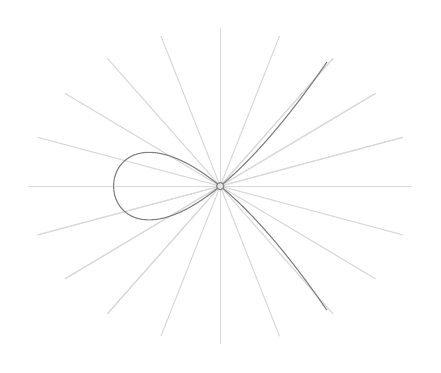
\begin{tikzpicture}
\begin{axis}[hide axis,xmin=-2,xmax=2,ymin=-2,ymax=2]
\newcommand{\RRR}{1.8}
\newcommand{\lineclr}{gray!30}
\draw[\lineclr] 
	({\RRR*cos(3.1415*0/10 r)},{\RRR*sin(3.1415*0/10 r)}) 
-- ({-\RRR*cos(3.1415*0/10 r)},{-\RRR*sin(3.1415*0/10 r)});
\draw[\lineclr] 
	({\RRR*cos(3.1415*1/10 r)},{\RRR*sin(3.1415*1/10 r)}) 
-- ({-\RRR*cos(3.1415*1/10 r)},{-\RRR*sin(3.1415*1/10 r)});
\draw[\lineclr] 
	({\RRR*cos(3.1415*2/10 r)},{\RRR*sin(3.1415*2/10 r)}) 
-- ({-\RRR*cos(3.1415*2/10 r)},{-\RRR*sin(3.1415*2/10 r)});
\draw[\lineclr] 
	({\RRR*cos(3.1415*3/10 r)},{\RRR*sin(3.1415*3/10 r)}) 
-- ({-\RRR*cos(3.1415*3/10 r)},{-\RRR*sin(3.1415*3/10 r)});
\draw[\lineclr] 
	({\RRR*cos(3.1415*4/10 r)},{\RRR*sin(3.1415*4/10 r)}) 
-- ({-\RRR*cos(3.1415*4/10 r)},{-\RRR*sin(3.1415*4/10 r)});
\draw[\lineclr] 
	({\RRR*cos(3.1415*1/10 r)},{-\RRR*sin(3.1415*1/10 r)}) 
-- ({-\RRR*cos(3.1415*1/10 r)},{\RRR*sin(3.1415*1/10 r)});
\draw[\lineclr] 
	({\RRR*cos(3.1415*2/10 r)},{-\RRR*sin(3.1415*2/10 r)}) 
-- ({-\RRR*cos(3.1415*2/10 r)},{\RRR*sin(3.1415*2/10 r)});
\draw[\lineclr] 
	({\RRR*cos(3.1415*3/10 r)},{-\RRR*sin(3.1415*3/10 r)}) 
-- ({-\RRR*cos(3.1415*3/10 r)},{\RRR*sin(3.1415*3/10 r)});
\draw[\lineclr] 
	({\RRR*cos(3.1415*4/10 r)},{-\RRR*sin(3.1415*4/10 r)}) 
-- ({-\RRR*cos(3.1415*4/10 r)},{\RRR*sin(3.1415*4/10 r)});
\draw[\lineclr] 
	({\RRR*cos(3.1415*1/10 r)},{\RRR*sin(3.1415*1/10 r)}) 
-- ({-\RRR*cos(3.1415*1/10 r)},{-\RRR*sin(3.1415*1/10 r)});
\draw[\lineclr] 
	({\RRR*cos(3.1415*2/10 r)},{\RRR*sin(3.1415*2/10 r)}) 
-- ({-\RRR*cos(3.1415*2/10 r)},{-\RRR*sin(3.1415*2/10 r)});
\draw[\lineclr] 
	({\RRR*cos(3.1415*3/10 r)},{\RRR*sin(3.1415*3/10 r)}) 
-- ({-\RRR*cos(3.1415*3/10 r)},{-\RRR*sin(3.1415*3/10 r)});
\draw[\lineclr] 
	(0,\RRR) 
-- (0,{-\RRR});
\newcommand{\curveclr}{gray}
  \addplot[domain=-1:0,\curveclr,samples=200]{sqrt(x^2+x^3)};%
  \addplot[domain=-1:0,\curveclr,samples=200]{-sqrt(x^2+x^3)};%
  \addplot[domain=0:1,\curveclr]{sqrt(x^2+x^3)};%
  \addplot[domain=0:1,\curveclr]{-sqrt(x^2+x^3)};%
  \fill[gray!20,draw=gray] (axis cs:0,0) circle (1.3pt);
\end{axis}
\end{tikzpicture}
\end{document}

\end{center}
Suppose that \(K\) is a field extension of \(k(C)\), say \(K=k(C)(\alpha)\) given by extending by an element \(\alpha\).
We want to draw a curve \(D\) so that \(K=k(D)\).

If \(\alpha\) is transcendental, then \(k(C)(\alpha) \cong k(C)(z)\) for some abstract variable \(z\).
But \(k(C)\) is already a field of rational functions of two variables \(x,y\), quotiented out to enforce the relation \(p(x,y)=0\).
So \(K\) is just the rational functions on the ``cylinder'' \(C \times k\) inside \(3\)-dimensional space, with variables \(x,y,z\); our cylinder has the equation \(p(x,y)=0\), independent of \(z\).
\begin{center}
\includegraphics[width=4cm]{cylinder-on-curve}
\end{center}
Suppose instead that \(\alpha\) is algebraic, say satisfying a polynomial equation \(f(z)=0\) with \(f(z)\) a polynomial with coefficients from \(k(C)\).
So each coefficient of \(f(z)\) is itself a rational function on \(C\).
Each such function is expressible as a rational function of \(x,y\).
Clearing denominators, we get a polynomial equation \(f(x,y,z)=0\) with coefficients in the underlying field \(k\).
The solutions form a surface in \(3\)-dimensional space.
But the resulting surface depends on how we pick out rational functions of \(x,y\) to represent our coefficients of \(f(z)\) from \(k(C)\).
So in fact we have to restrict our \(x,y\) variables to lie in \(C\), i.e. we consider the \emph{curve} \(D\) cut out by the equations \(p(x,y)=f(x,y,z)=0\).
\begin{center}
\includegraphics[width=4cm]{cylinder-on-curve-2}
\end{center}
The map \(\pr{x,y,z} \in D \mapsto \pr{x,y} \in C\) is regular.

We wonder now whether there is a \(k(C)\)-root to \(f(z)=0\), say \(\beta\).
This \(\beta\) is in \(k(C)\), so a rational function on \(C\), so that \(f(\beta)=0\).
So this is a rational map \(z=\beta(x,y)\) from \(C\) to \(D\), lifting the curve \(C\) up from the plane into space, tracing out \(D\) on the cylinder.
In particular, there is no such map if \(D\) is irreducible and \(D \to C\) is many to one:
\begin{center}
\includegraphics[width=4cm]{cylinder-on-curve-3}
\end{center}
So in such a case, \(k(C) \subset k(D)\) is a nontrivial field extension.
We get a picture giving some intuition for nontrivial algebraic field extensions: typically we expect to see an irreducible curve \(D\) mapping to a curve \(C\) by a many-to-one map.
The Galois group of \(k(D)/k(C)\) swaps strands of the curve \(D\) up and down in the picture, so each point of \(D\) remains over the same point of \(C\) as before the swap.

The story continues similarly in higher dimensions: a transcendental extension increases dimension as a ``cylinder'', while an algebraic extension, say of degree \(n\), preserves dimension, giving a new geometric object, sitting inside such a ``cylinder'', mapping regularly to the old one, by an \(n\)-to-\(1\) map.

   
\section{Rational curves}
Recall that the \emph{degree}\SubIndex{degree!of field extension} of a field extension \(k \subset K\), denoted \([K:k]\), is the smallest integer \(n\) so that there are \(n\) elements \(\alpha_1, \alpha_2, \dots, \alpha_n\) of \(K\) so that every element of \(K\) is a linear combination \(\sum a_j \alpha_j\) with coefficients \(a_1, a_2, \dots, a_n\) in \(k\).
The degree of the field extension is infinite if there is no such integer \(n\).
\begin{problem}{algebraic.curves:degree.multiplies}
Suppose that \(k \subset K \subset L\) are field extensions.
Prove that \([L:k]=[L:K][K:k]\).
Note: this works even if one or more degree is infinite: let \(n\infty=\infty n = \infty \infty = \infty\) for any positive integer \(n\).
You have to prove these infinite degree cases as well.
\end{problem}
\begin{problem}{algebraic.curves:degree.one}
Prove that a field extension is an isomorphism if and only if it has degree one.
\end{problem}
\begin{answer}{algebraic.curves:degree.one}
Take a basis consisting of one element \(\alpha \in K\).
Then \(1 \in K\) is somehow a multiple \(1=a \alpha\) for some \(a \in k\) so \(\alpha=1/a \in k\).
Any element \(\beta\) of \(K\) is \(\beta=c \alpha\) for some \(c \in k\) so \(\beta \in k\).
\end{answer}
\begin{problem}{algebraic.curves:find.degree}
Suppose that \(p(x)\) is an irreducible polynomial over a field \(k\).
Let \(K\defeq k[x]/(p(x))\).
Prove that \([K:k]\) is the degree of \(p(x)\).
\end{problem}
\begin{answer}{algebraic.curves:find.degree}
Let \(n\) be the degree of \(p(x)\).
We write each element \(b(x)\) in  \(k[x]\) as a polynomial, but if the polynomial has degree \(n\) or more, rewrite it as \(b(x)=q(x)p(x)+r(x)\), quotient and remainder. Then every element of \(K\) is written as the remainder term, i.e. as a polynomial of degree at most \(n-1\).  Hence the elements \(1,x,\dots,x^{n-1}\) in \(k[x]\) map to a spanning set inside \(K\). If not a basis, then there must be some linear relation between them, i.e. a lower degree polynomial in \(x\) vanishing in \(K\), i.e. vanishing modulo \(p(x)\).
But then taking quotient and remainder, we see that this is not possible.
Hence \(K\) has a basis over \(k\) consisting of the images of \(1,x,x^2,\dots,x^{n-1}\) in \(k[x]\).
\end{answer}
\begin{problem}{algebraic.curves:infinitely.many.points.on.trace}
Prove that if \(u(t)\) is a nonconstant rational function over a field \(k\), then there are infinitely many values of \(u(t)\) as \(t\) varies over \(\bar{k}\).
In particular, \(k \subset k(u(t))\) is a transcendental extension.
\end{problem}
Recall that a curve \(C=(0=f(x,y))\) is \emph{irreducible}
\SubIndex{irreducible!polynomial}%
\SubIndex{reducible!polynomial}% 
\SubIndex{polynomial!irreducible}%
\SubIndex{polynomial!reducible}
if \(f(x,y)\) is irreducible as a polynomial.
\begin{theorem}
An irreducible plane algebraic curve \(C\) over a field \(k\) is rational just when there is a nonconstant rational map \(k \to C\).
In other words, \(C\) is rational just when there are rational functions \(x(t),y(t)\), not both constant, for which the point \((x(t),y(t))\) lies in \(C\) for all \(t\) in the algebraic closure of the field for which \(x(t)\) and \(y(t)\) are both defined.
\end{theorem}
\begin{proof}
If our curve \(C\) is rational then by definition \(C\) is birational to a line, so there is such a map.
Suppose on the other hand that there is such a map \(k \to C\), say written as \(t \in k \mapsto (x(t),y(t)) \in C\) with
\[
f(x(t),y(t))=0
\]
for some rational functions \(x(t), y(t)\), not both constant.
As we vary \(t\) through \(\bar{k}\), the moving point \((x(t),y(t))\) moves through infinitely many different points of the plane.
Take a rational function on \(C\), say \(g(x,y)=b(x,y)/c(x,y)\).
Then \(c(x,y)\ne 0\) at all but finitely points of \(C\).
(Note that this requires that our curve \(C\) is irreducible, as otherwise we might have \(g(x,y)\) vanishing on a component of \(C\).)
So at infinitely many values of \(t\), \(g(x(t),y(t))\) is defined.
We map \(g(x,y) \in k(C) \mapsto g(x(t),y(t)) \in k(t)\), a morphism of fields. 
The image is some subfield \(K=k(x(t),y(t)) \subset k(t)\).
The result follows from the following theorem applied to \(K\).
\end{proof}
\begin{theorem}[L\"uroth's theorem]\define{Luroth's theorem@L\"uroth's theorem}\define{theorem!Luroth@L\"uroth}
Suppose that \(k \subset K \subset k(t)\) is a finitely generated extension of a field \(k\), where \(t\) is an abstract variable.
Then \(K=k(f(t))\) is generated by a single rational function \(f(t)\) in \(k(t)\).
In particular, either \(K=k\) (if \(f(t)\) is a constant function) or \(K\) is isomorphic to \(k(t)\) by \(t \mapsto f(t)\).
\end{theorem}
The proof of this theorem requires a lemma:
\begin{lemma}
Take a nonconstant rational function \(f(x)=b(x)/c(x)\), with \(b(x), c(x)\) coprime, over a field \(k\).
Then, as a polynomial in a variable \(y\) with coefficients in \(k(f(x))\), the expression
\[
f(x)c(y)-b(y) 
\]
in \(k(f(x))[y]\) is irreducible.
\end{lemma}
\begin{proof}
This expression is not zero, because it is nonconstant in \(x\).
It vanishes at \(y=x\).
Hence \(x\) satisfies this polynomial (in \(y\)) expression with coefficients in \(k(f(x))\).
So \(k(x)\) is an algebraic extension of \(k(f(x))\).
Since \(k(x)\) is transcendental over \(k\), \(k(f(x))\) is transcendental over \(k\).
So \(f(x)\) solves no polynomial equation over \(k\).
Take an abstract variable \(t\). 
Map \(k(t,y) \to k(f(x),y)\) by \(t \mapsto f(x)\).
This map is an isomorphism of fields.
Similarly \(k[t,y] \to k[f(x),y]\) is an isomorphism of rings.
In order to prove that \(tc(y)-b(y)\) is irreducible in \(k(t)[y]\), it suffices to prove that it is irreducible in \(k[t,y]\), i.e. clear \(t\) from denominators, by Gauss's lemma (proposition~\vref{proposition:Gauss.lemma}).
If we can factor \(tc(y)-b(y)=g(t,y)h(t,y)\) in \(k[t,y]\) then one of \(g(t,y)\) or \(h(t,y)\) has degree \(1\) in \(t\), since the product does, and so one of \(g(t,y)\) or \(h(t,y)\) has degree zero in \(t\), depending only on \(y\), say \(g(t,y)=g(y)\).
Then \(g(y)h(t,y)=tc(y)-b(y)\), so \(g(y)\) divides \(tc(y)-b(y)\), and since \(t\) is an abstract variable, \(g(y)\) divides \(b(y)\) and \(c(y)\), which are coprime, so \(g(y)\) is a nonzero constant.
\end{proof}
We now prove L\"uroth's theorem:
\begin{proof}
For each element \(f(t)=b(t)/c(t)\) in \(K\), let \(n\) be the  larger of the degrees of \(b(t),c(t)\).
Pick an element \(f(t)=b(t)/c(t)\) in \(K\), not in \(k\), for which the value of \(n\) is as small as possible.
By the previous lemma, the polynomial \(B(y)=f(x)c(y)-b(y)\) is irreducible in \(k(f(x))[y]\), so the map
\[
x,y \in k(f(x))[y]/(B(y)) \mapsto x,x \in k(x)
\]
is an isomorphism of fields and \([k(x):k(f(x))]=n\).
The expression \(B(y)\) is the polynomial in \(K[y]\) of smallest positive \(y\)-degree which is satisfied by \(y=x\), since a smaller degree one would give a smaller value for \(n\).
Indeed the \(y\)-degree of \(B(y)\) is \(n\).
In particular, \(B(y)\) is also irreducible in \(K[y]\) and the map
\[
x,y \in K[y]/(B(y)) \mapsto x,x \in k(x)
\]
is an isomorphism.
In particular, \([k(x):K]=n\).
But
\begin{align*}
n
&=[k(x):k(f(x))],
\\
&=[k(x):K][K:k(f(x))],
\\
&=n[K:k(f(x))]
\end{align*}
so \([K:k(f(x))]=1\).
\end{proof}   